\documentclass[11pt]{article}
\usepackage[margin=1in]{geometry}
\usepackage[T1]{fontenc}
\usepackage{tikz}
\usepackage[american]{circuitikz}
\usepackage{longtable}
\usepackage{hyperref}
\title{rlc\_bandpass}
\author{Generated by mixedsig2cad}
\date{\today}
\begin{document}
\maketitle
\section{Readable Circuit}
\begin{circuitikz}[american voltages, scale=1, transform shape]
  \draw (8.38,-7.75) to[R,l={50},t={R1}] (9.65,-7.75);
  \draw (13.59,-9.02) to[R,l={1k},t={R2}] (13.59,-10.29);
  \draw (11.68,-9.02) to[C,l={100n},t={C1}] (11.68,-10.29);
  \draw (11.30,-7.75) to[L,l={10m},t={L1}] (12.57,-7.75);
  \draw (5.59,-7.87) to[V,l={AC 1},t={V1}] (5.59,-9.40);
  \draw (13.59,-11.43) node[ground] {};
  \draw (5.59,-10.54) node[ground] {};
  \draw (11.68,-11.43) node[ground] {};
  \draw (11.68,-10.29) -- (11.68,-11.43);
  \draw (5.59,-9.40) -- (5.59,-10.54);
  \draw (13.59,-10.29) -- (13.59,-11.43);
  \draw (11.30,-7.75) -- (9.65,-7.75);
  \draw (11.68,-9.02) -- (12.57,-9.02);
  \draw (13.59,-7.75) -- (12.57,-7.75);
  \draw (13.59,-9.02) -- (13.59,-7.75);
  \draw (12.57,-9.02) -- (12.57,-7.75);
  \draw (5.59,-7.75) -- (8.38,-7.75);
  \draw (5.59,-7.87) -- (5.59,-7.75);
  \fill (12.57,-7.75) circle (1.2pt);
  \node[font=\scriptsize] at (9.02,-7.37) {R1};
  \node[font=\scriptsize] at (9.02,-8.13) {50};
  \node[font=\scriptsize] at (13.08,-9.40) {R2};
  \node[font=\scriptsize] at (14.10,-9.40) {1k};
  \node[font=\scriptsize] at (11.68,-9.27) {C1};
  \node[font=\scriptsize] at (11.68,-10.03) {100n};
  \node[font=\scriptsize] at (11.94,-7.37) {L1};
  \node[font=\scriptsize] at (11.94,-8.00) {10m};
  \node[font=\scriptsize] at (5.21,-7.75) {V1};
  \node[font=\scriptsize] at (5.33,-9.53) {AC 1};
  \node[font=\scriptsize] at (13.59,-11.94) {GND};
  \node[font=\scriptsize] at (5.59,-11.05) {GND};
  \node[font=\scriptsize] at (11.68,-11.94) {GND};
  \node[font=\scriptsize] at (5.59,-7.75) {vin};
  \node[font=\scriptsize] at (12.57,-7.75) {n2};
  \node[font=\scriptsize] at (9.65,-7.75) {n1};
\end{circuitikz}
\section{Literal KiCad Reference}
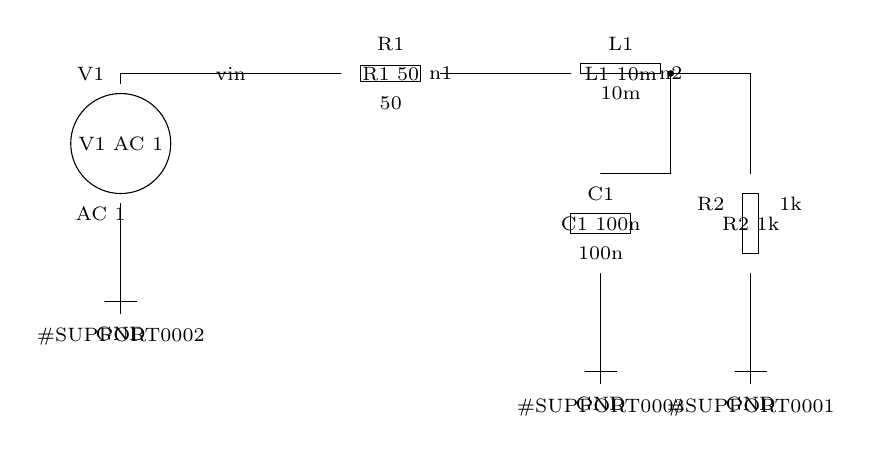
\begin{tikzpicture}[x=0.1cm,y=-0.1cm,line cap=round,line join=round]
  \draw (116.84,102.87) -- (116.84,114.30);
  \draw (55.88,93.98) -- (55.88,105.41);
  \draw (135.89,102.87) -- (135.89,114.30);
  \draw (113.03,77.47) -- (96.52,77.47);
  \draw (116.84,90.17) -- (125.73,90.17);
  \draw (135.89,77.47) -- (125.73,77.47);
  \draw (135.89,90.17) -- (135.89,77.47);
  \draw (125.73,90.17) -- (125.73,77.47);
  \draw (55.88,77.47) -- (83.82,77.47);
  \draw (55.88,78.74) -- (55.88,77.47);
  \fill (125.73,77.47) circle (1.2pt);
  \draw (86.36,76.45) rectangle (93.98,78.49);
  \node[font=\scriptsize,align=center] at (90.17,77.47) {R1 50};
  \draw (134.87,92.71) rectangle (136.91,100.33);
  \node[font=\scriptsize,align=center] at (135.89,96.52) {R2 1k};
  \draw (113.03,95.25) rectangle (120.65,97.79);
  \node[font=\scriptsize,align=center] at (116.84,96.52) {C1 100n};
  \draw (114.30,76.20) rectangle (124.46,77.47);
  \node[font=\scriptsize,align=center] at (119.38,77.47) {L1 10m};
  \draw (55.88,86.36) circle (6.35);
  \node[font=\scriptsize,align=center] at (55.88,86.36) {V1 AC 1};
  \draw (135.89,114.30) -- (135.89,116.84);
  \draw (133.89,115.34) -- (137.89,115.34);
  \node[font=\scriptsize] at (135.89,119.84) {\#SUPPORT0001};
  \draw (55.88,105.41) -- (55.88,107.95);
  \draw (53.88,106.45) -- (57.88,106.45);
  \node[font=\scriptsize] at (55.88,110.95) {\#SUPPORT0002};
  \draw (116.84,114.30) -- (116.84,116.84);
  \draw (114.84,115.34) -- (118.84,115.34);
  \node[font=\scriptsize] at (116.84,119.84) {\#SUPPORT0003};
  \node[font=\scriptsize] at (90.17,73.66) {R1};
  \node[font=\scriptsize] at (90.17,81.28) {50};
  \node[font=\scriptsize] at (130.81,93.98) {R2};
  \node[font=\scriptsize] at (140.97,93.98) {1k};
  \node[font=\scriptsize] at (116.84,92.71) {C1};
  \node[font=\scriptsize] at (116.84,100.33) {100n};
  \node[font=\scriptsize] at (119.38,73.66) {L1};
  \node[font=\scriptsize] at (119.38,80.01) {10m};
  \node[font=\scriptsize] at (52.07,77.47) {V1};
  \node[font=\scriptsize] at (53.34,95.25) {AC 1};
  \node[font=\scriptsize] at (135.89,119.38) {GND};
  \node[font=\scriptsize] at (55.88,110.49) {GND};
  \node[font=\scriptsize] at (116.84,119.38) {GND};
  \node[font=\scriptsize] at (69.85,77.47) {vin};
  \node[font=\scriptsize] at (125.73,77.47) {n2};
  \node[font=\scriptsize] at (96.52,77.47) {n1};
\end{tikzpicture}
\section{Reference Summary}
\begin{longtable}{p{0.16\linewidth}p{0.18\linewidth}p{0.30\linewidth}p{0.22\linewidth}}
\textbf{Ref} & \textbf{Kind} & \textbf{Value / Model} & \textbf{Nodes}\\
\hline
V1 & V & AC 1 & vin, 0\\
R1 & R & 50 & vin, n1\\
L1 & L & 10m & n1, n2\\
C1 & C & 100n & n2, 0\\
R2 & R & 1k & n2, 0\\
\end{longtable}

\paragraph{Analyses}
\begin{itemize}
  \item \texttt{ac dec 40 10 100k}
\end{itemize}
\section{Design Notes}
\subsection*{Overview}
This generated example captures the rlc bandpass circuit using voltage sources, resistors, inductors, and related support parts.

\subsection*{Operating Notes}
\begin{itemize}
  \item Primary simulation commands: ac dec 40 10 100k.
  \item Component count: 5 active entries in the shared CircuitSpec.
  \item Named nets to review during edits: n1, n2, vin.
\end{itemize}
\subsection*{Design Notes To Edit}
\begin{itemize}
  \item Replace these starter notes with intended operating limits, tuning guidance, and simulation expectations.
  \item Record any KiCad-specific layout conventions that should stay aligned with the generated schematic.
  \item Add usage notes for the ngspice analyses that matter for this example.
\end{itemize}
\end{document}
